\begin{frame}
  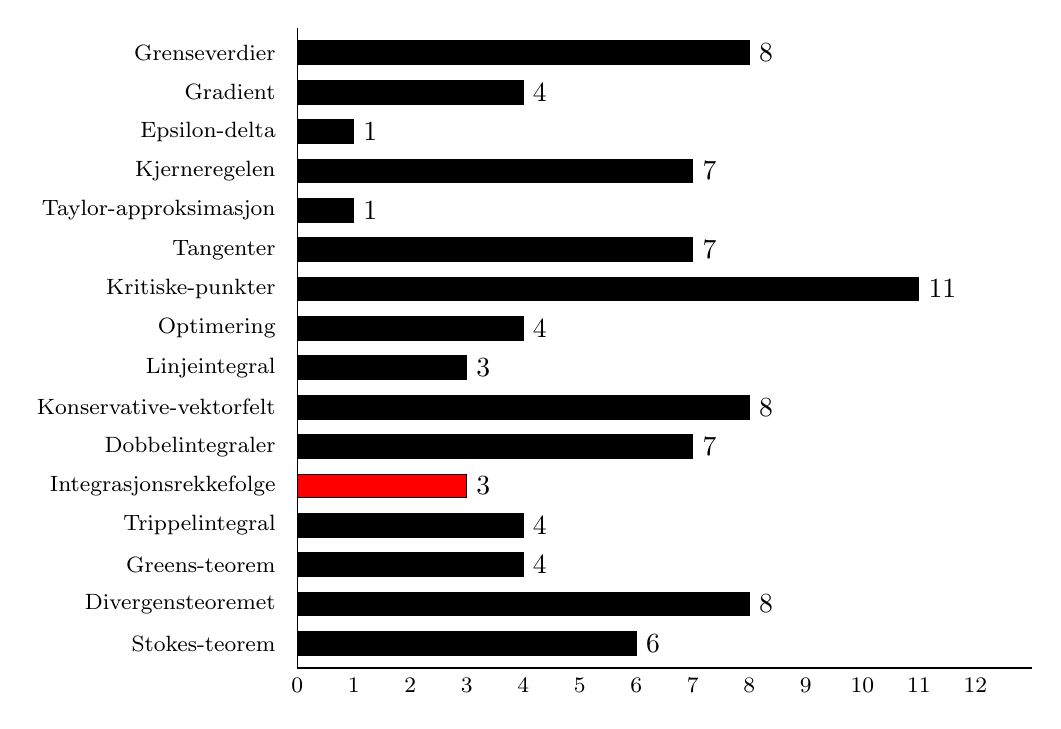
\begin{tikzpicture}
    \begin{axis}[ xbar=0pt, /pgf/bar shift=0pt, legend style={ legend columns=4,
        at={(xticklabel cs:0.5)}, anchor=north, draw=none }, ytick={0,...,15},
      ytick style={draw=none},% <- added
      axis y line*=none, axis x line*=bottom, tick label
      style={font=\footnotesize}, legend style={font=\footnotesize}, label
      style={font=\footnotesize}, xtick style={draw=none},% <- added
      xtick={0,1,...,12}, width=.9\textwidth, bar width=3mm, y dir = reverse,
      xmin=0, xmax=13, area legend,
      y=5mm, enlarge y limits={abs=0.625},
      style={text=black}, every axis plot/.append style={fill},
      nodes near coords, nodes near coords,
      yticklabels={%
        {\topicref{Grenseverdier}},
        {\topicref{Gradient}},
        {\topicref{Epsilon-delta}},
        {\topicref{Kjerneregelen}},
        {\topicref{Taylor-approksimasjon}},
        {\topicref{Tangenter}},
        {\topicref{Kritiske-punkter}},
        {\topicref{Optimering}},
        {\topicref{Linjeintegral}},
        {\topicref{Konservative-vektorfelt}},
        {\topicref{Dobbelintegraler}},
        {\topicref{Integrasjonsrekkefolge}},
        {\topicref{Trippelintegral}},
        {\topicref{Greens-teorem}},
        {\topicref{Divergensteoremet}},
        {\topicref{Stokes-teorem}}}]
      \addplot[fill=black] coordinates {(8,0)};
      \addplot[fill=black] coordinates {(4,1)};
      \addplot[fill=black] coordinates {(1,2)};
      \addplot[fill=black] coordinates {(7,3)};
      \addplot[fill=black] coordinates {(1,4)};
      \addplot[fill=black] coordinates {(7,5)};
      \addplot[fill=black] coordinates {(11,6)};
      \addplot[fill=black] coordinates {(4,7)};
      \addplot[fill=black] coordinates {(3,8)};
      \addplot[fill=black] coordinates {(8,9)};
      \addplot[fill=black] coordinates {(7,10)};
      \addplot[fill=red] coordinates {(3,11)};
      \addplot[fill=black] coordinates {(4,12)};
      \addplot[fill=black] coordinates {(4,13)};
      \addplot[fill=black] coordinates {(8,14)};
      \addplot[fill=black] coordinates {(6,15)};
    \end{axis}
  \end{tikzpicture}
\end{frame}

\begin{frame}
  \subsection{Integrasjonsrekkefølge}\label{subsec:Integrasjonsrekkefolge}
  \begin{oppgave}{V2017, Oppgave 3}
    Skisser integrasjonsområdet for
    %
    $\displaystyle
      \int_0^1 \int_{\sqrt{x}}^1 f(x,y) \dy \dx,
    $
    %
    og bytt integrasjonsrekkefølgen til $\dx \dy$.
  \end{oppgave}
    \centerline{%
    \only<1>{\includegraphics[scale=0.8]{../img/dobbelIntegral1}}
    \only<2>{\includegraphics[scale=0.8]{../img/dobbelIntegral2}}
    \only<3>{\includegraphics[scale=0.8]{../img/dobbelIntegral3}}
    \only<4>{\includegraphics[scale=0.8]{../img/dobbelIntegral4}}
    \only<5>{\includegraphics[scale=0.8]{../img/dobbelIntegral5}}
    \only<6>{\includegraphics[scale=0.8]{../img/dobbelIntegral6}}
  }
  \vspace{-0.5cm}
  \begin{equation*}
      \int_{\only<1>{x = 0}\only<2>{\textcolor{blue}{x=0}}\only<3->{x=0}}^{\only<1-4>{x = 1}\only<5>{\textcolor{blue}{x=1}}\only<6->{x=1}} \int_{\only<1-2>{y = \sqrt{x}}\only<3>{\textcolor{blue}{y=\sqrt{x}}}\only<4->{y=\sqrt{x}}}^{\only<1-3>{y = 1}\only<4>{\textcolor{blue}{y=0}}\only<5->{y=0}} f(x,y) \dy \dx,
  \end{equation*}
\end{frame}

\begin{frame}
  \begin{oppgave}{V2017, Oppgave 3}
    Skisser integrasjonsområdet for
    %
    $\displaystyle
      \int_0^1 \int_{\sqrt{x}}^1 f(x,y) \dy \dx,
    $
    %
    og bytt integrasjonsrekkefølgen til $\dx \dy$.
  \end{oppgave}
  \centerline{%
    \only<1>{\includegraphics[scale=0.8]{../img/dobbelIntegral10}}
    \only<2>{\includegraphics[scale=0.8]{../img/dobbelIntegral11}}
    \only<3>{\includegraphics[scale=0.8]{../img/dobbelIntegral12}}
    \only<4>{\includegraphics[scale=0.8]{../img/dobbelIntegral13}}
    \only<5>{\includegraphics[scale=0.8]{../img/dobbelIntegral14}}
    \only<6-7>{\includegraphics[scale=0.8]{../img/dobbelIntegral15}}
  }
  \only<1-7>{
  \vspace{-0.5cm}
  \begin{equation*}
    \int_0^1 \int_{\sqrt{x}}^{1} f(x,y) \dy \dx
    =
    \int_{\only<1-4>{?}\only<5>{\textcolor{red}{y=0}}\only<6->{0}}^{\only<1-5>{?}\only<6>{\textcolor{red}{y=1}}\only<7>{1}} \int_{\only<1>{?}\only<2>{\textcolor{blue}{x=0}}\only<3->{0}}^{\only<1-2>{?}\only<3>{\textcolor{blue}{x=y^2}}\only<4->{y^2}} f(x,y) \dx \dy
  \end{equation*}}%
  \only<8>{
  Har at $0 \leq x \leq 1$ og $\sqrt{x} \leq y \leq 1$. Dette fører til at
  %
  \begin{equation*}
    \sqrt{0} \leq y \leq 1
  \end{equation*}
  %
  Ved å kvadrere $\sqrt{x} \leq y \leq 1$ får vi $x \leq y^2 \leq 1$. Videre vet
  vi at $0 \leq x$ slik at
  %
  \begin{equation*}
    0 \leq x \leq y^2
  \end{equation*}}
\end{frame}

%%% Local Variables:
%%% mode: latex
%%% TeX-master: "main"
%%% End:
